\documentclass[11pt,a4paper]{article}
\usepackage[margin=2.2cm]{geometry}
\usepackage{lmodern}
\usepackage{amsmath,amssymb}
\usepackage{booktabs,array,tabularx}
\usepackage{enumitem}
\usepackage{siunitx}
\usepackage{float}
\usepackage{tikz}
\usetikzlibrary{arrows.meta,positioning}
\usepackage{xurl}
\usepackage[hidelinks]{hyperref}
\numberwithin{equation}{section}
\newcommand{\Fd}{F_4}
\newcommand{\Teff}{T_{\text{eff}}}
\newcommand{\R}{\mathbb{R}}
\newcolumntype{Y}{>{\raggedright\arraybackslash}X}

\title{A black-box function for Gaussian-process emulation\\and Bayesian optimisation of the CNVI ranking\\[4pt]
\large Definition for approval (no code written yet)}
\author{EST project, Climate--Nutrition Vulnerability Index}
\date{18 November 2026}

\begin{document}
\maketitle
\tableofcontents

\section{Question}
The main result of the report is that wheat is the most vulnerable of the nine crops under both country
weightings. That claim has so far been tested one parameter at a time: in the 14 tests that change a physical
crop parameter (heat threshold, heat slope, $K_y$), wheat stays first every time. One-at-a-time tests cannot show
what happens when several uncertain parameters move \emph{together}. This analysis asks:
\begin{enumerate}[label=\textbf{Q\arabic*.}]
\item \textbf{Worst case (optimisation).} Within the documented literature ranges, varied jointly, how close can
the runner-up get to wheat, and can wheat lose first place?
\item \textbf{Prediction.} Over the whole parameter box, where is wheat's lead small, what fraction of the box keeps
wheat first, and which parameters matter most?
\end{enumerate}
Q1 is answered with Bayesian optimisation (BO), Q2 with the Gaussian-process (GP) surrogate that BO builds.
The analysis is an additional robustness check. It does not change any result in the report.

\section{The black-box function}\label{sec:bb}

\subsection{Inputs}
The input is a vector $\theta\in\Theta\subset\R^6$ of the crop parameters that the report flags as uncertain
(fits, proxies, or chamber values). Each range is one that the report already tests one at a time
(\texttt{config.PARAM\_RANGES} and the robustness table), so no new range is introduced.

\begin{table}[h]\centering\small
\caption{Inputs of the black box. Nominal values reproduce the published index.}\label{tab:inputs}
\begin{tabularx}{\linewidth}{@{}l Y l l l@{}}
\toprule
& Meaning & Crops affected & Nominal & Range \\
\midrule
$\theta_1$ & Shift of the heat threshold $T_{\text{crit}}$, \si{\celsius} & all nine & 0 & $[-2,\,+3]$ \\
$\theta_2$ & Extra threshold shift for the new legumes (chamber vs model thresholds), \si{\celsius}
           & chickpea, lentil, bean, groundnut & 0 & $[0,\,+3]$ \\
$\theta_3$ & Multiplier on the heat slope $s_T$ (chamber $\to$ field) & same four legumes & 1.0 & $[0.7,\,1.0]$ \\
$\theta_4$ & Rapeseed heat slope $s_T$ (proxy), \si{\per\celsius} & rapeseed & 0.10 & $[0.07,\,0.18]$ \\
$\theta_5$ & Rice $K_y$ (proxy; FAO gives none) & rice & 1.25 & $[1.0,\,1.5]$ \\
$\theta_6$ & Position of the new-crop $K_y$ between its low ($-1$) and high ($+1$) published values
           & chickpea, lentil, bean, rapeseed & 0 & $[-1,\,+1]$ \\
\bottomrule
\end{tabularx}
\end{table}
\noindent For $\theta_6$, each affected crop $c$ gets
\begin{equation}
K_{y,c}(\theta_6)=K^{0}_{y,c}+\begin{cases}\theta_6\,(K^{\text{high}}_{y,c}-K^{0}_{y,c}) & \theta_6\ge 0\\
|\theta_6|\,(K^{\text{low}}_{y,c}-K^{0}_{y,c}) & \theta_6<0\end{cases}
\end{equation}
with (low, nominal, high) = chickpea (0.67, 0.88, 1.15), lentil (0.87, 1.00, 1.15), bean (0.60, 1.15, 1.40),
rapeseed (0.85, 0.90, 0.95). The optimiser works on the unit cube: $x_j=(\theta_j-a_j)/(b_j-a_j)\in[0,1]$ for
range $[a_j,b_j]$.

Not varied: the climate data, crop maps, calendars, importance weights (already covered by the existing Monte Carlo
over weightings) and the parameters of the established crops beyond $\theta_1$ and $\theta_5$.

\subsection{Evaluation: what one call of $f(\theta)$ does}
Each call reruns the part of the pipeline that depends on $\theta$, with every other input fixed at the
published 2001--2024 values.
\begin{enumerate}[leftmargin=*]
\item \textbf{Heat hazard with shifted thresholds.} For crop $c$ the threshold becomes
$\tau_c = T_{\text{crit},c}+\theta_1+\theta_2\,\mathbf{1}[c\in\text{legumes}]$ (slope unchanged, as in the existing
threshold tests). Per cell $i$ and season-year $t$,
\begin{equation}\label{eq:heat}
\text{HEAT}_{c,i,t}(\tau_c)=\frac{\sum_m w_{m}\,\max\bigl(0,\;\Teff{}_{,i,m}-\tau_c\bigr)}{\sum_m w_{m}},\qquad
\Teff=\tfrac12(T_{\text{mean}}+T_{\max}),
\end{equation}
over the monthly flowering weights $w_m$ (45--70\% of the season), exactly as in \texttt{04\_hazards.py}.
\item \textbf{National levels.} $L_{\text{heat}}$ is the area-weighted, 2001--2024 mean of Eq.~\ref{eq:heat}
(\path{05_country_series.py}). The water level $L_{\text{water}}$ does not depend on $\theta$ and is reused.
\item \textbf{Sensitivities.} $s_{T,c}$ and $K_{y,c}$ are set from $\theta_3$--$\theta_6$ and re-normalised over the
crops: $S_T=s_T/\max s_T$, $S_P=K_y/\max K_y$. (If rice $K_y=1.5$ or bean $K_y=1.4$ the maximum changes, so
every crop's $S_P$ moves.)
\item \textbf{Index.} Exposures are re-normalised over the 59 pairs, $E=L/\max L$, and
$\Fd=\tfrac12(E_{\text{heat}}S_T+E_{\text{water}}S_P)\,\tilde I$ per pair (\texttt{08\_index.py},
\texttt{calculate\_indices}).
\item \textbf{Crop scores.} $\Fd^{w}(c;\theta)$ for $w\in\{\text{eq},\text{pw}\}$: equal-weighted and
production-weighted means over each crop's countries.
\end{enumerate}

\subsection{Output}
\begin{equation}\label{eq:f}
\boxed{\;f(\theta)=\min_{w\in\{\text{eq},\,\text{pw}\}}\Bigl[\ln \Fd^{w}(\text{wheat};\theta)\;-\;
\ln\max_{c\neq\text{wheat}}\Fd^{w}(c;\theta)\Bigr]\;}
\end{equation}
$f$ is the log-ratio of wheat's score to the best other crop's score, taken under the less favourable of the two
weightings.
\begin{itemize}
\item $f>0$: wheat is first under both weightings; $e^{f}$ is its lead (e.g.\ $e^{f}=1.5$ means 50\% ahead).
\item $f<0$: some crop overtakes wheat under at least one weighting. The minimising $\theta$ says which
parameter combination does it.
\item At the nominal $\theta^{0}$: equal-weighted $\ln(0.05634/0.02967)=0.641$ (runner-up maize);\\
production-weighted $\ln(0.06964/0.02328)=1.096$ (runner-up bean); hence $f(\theta^0)=0.641$.
\end{itemize}
The log-ratio is chosen over a plain difference because it is scale-free: re-normalising by maxima rescales all
scores together, which leaves the ratio unchanged.

\subsection{Why it is treated as a black box}
\begin{itemize}
\item \textbf{No closed form in $\theta$.} $\theta_1,\theta_2$ act through $\max(0,\cdot)$ on monthly values in tens
of thousands of cells over 24 years, then through area weighting and maxima over pairs.
\item \textbf{Not differentiable.} Maxima (over crops in Eq.~\ref{eq:f}, and in each normalisation) create kinks, so
gradient methods are unsuitable.
\item \textbf{Costly.} A non-integer threshold shift needs the monthly hazard loop again (the pipeline stores only
integer shifts $-2,\dots,+3$). Rereading the monthly rasters takes minutes per call. A cache of the
flowering-window monthly $\Teff$ per cell (exact, not an approximation) would cut a call to seconds; if built, it
makes a large reference search affordable, which is used only to check the BO answer (Section~\ref{sec:checks}).
\item \textbf{Deterministic.} The same $\theta$ always gives the same $f$; there is no observation noise.
\end{itemize}

\begin{figure}[h]\centering
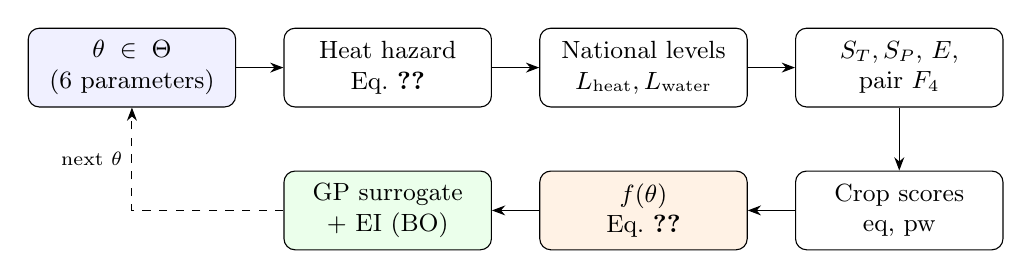
\begin{tikzpicture}[node distance=4mm and 6mm, box/.style={draw,rounded corners,align=center,font=\small,
  minimum height=10mm,text width=24mm}, >={Stealth}]
\node[box,fill=blue!6] (th) {$\theta\in\Theta$\\(6 parameters)};
\node[box,right=of th] (hz) {Heat hazard\\Eq.~\ref{eq:heat}};
\node[box,right=of hz] (lv) {National levels\\$L_{\text{heat}},L_{\text{water}}$};
\node[box,right=of lv] (ix) {$S_T,S_P$, $E$,\\ pair $\Fd$};
\node[box,below=8mm of ix] (cs) {Crop scores\\eq, pw};
\node[box,left=of cs,fill=orange!10] (f) {$f(\theta)$\\Eq.~\ref{eq:f}};
\node[box,left=of f,fill=green!8] (gp) {GP surrogate\\+ EI (BO)};
\draw[->] (th)--(hz); \draw[->] (hz)--(lv); \draw[->] (lv)--(ix); \draw[->] (ix)--(cs); \draw[->] (cs)--(f);
\draw[->] (f)--(gp); \draw[->,dashed] (gp) -| node[pos=0.75,left,font=\scriptsize]{next $\theta$} (th);
\end{tikzpicture}
\caption{One evaluation of the black box (top row and crop scores) and the BO loop that chooses the next input.}
\end{figure}

\section{Gaussian-process surrogate}
Given $n$ evaluations $\mathcal D_n=\{(x_k,y_k)\}_{k=1}^{n}$ with $y_k=f(x_k)$, outputs are standardised
($\bar y$, $s_y$) and modelled as $f\sim\mathcal{GP}(0,k)$ with a Mat\'ern-5/2 kernel and one length scale per
input (automatic relevance determination):
\begin{equation}
k(x,x')=\sigma_f^2\Bigl(1+\sqrt5\,r+\tfrac53 r^2\Bigr)e^{-\sqrt5\,r},\qquad
r^2=\sum_{j=1}^{6}\frac{(x_j-x'_j)^2}{\ell_j^2}.
\end{equation}
Mat\'ern-5/2 is used rather than the squared-exponential kernel because $f$ has kinks. With
$K=[k(x_a,x_b)]+\sigma_n^2 I$ and $k_n(x)=[k(x,x_1),\dots,k(x,x_n)]^\top$, the posterior at any $x$ is
\begin{align}
\mu_n(x)&=k_n(x)^\top K^{-1}y,\label{eq:mu}\\
\sigma_n^2(x)&=k(x,x)-k_n(x)^\top K^{-1}k_n(x).\label{eq:sigma}
\end{align}
Because $f$ is deterministic, $\sigma_n^2$ is a small fixed nugget ($10^{-6}$ on the standardised scale) for
numerical stability only. The hyperparameters $\psi=(\sigma_f,\ell_1,\dots,\ell_6)$ maximise the log marginal
likelihood
\begin{equation}
\log p(y\mid X,\psi)=-\tfrac12\,y^\top K^{-1}y-\tfrac12\log|K|-\tfrac n2\log 2\pi,
\end{equation}
with $\ell_j\in[0.05,10]$ on the unit cube and 10 random restarts of L-BFGS-B. Implementation: NumPy/SciPy only
(Cholesky solves), so no new dependency is added to \texttt{requirements.txt}.

\section{Bayesian optimisation}
\paragraph{Objective.} $x^\star=\arg\min_{x\in[0,1]^6} f(x)$ (the worst case for wheat's lead).

\paragraph{Acquisition.} Expected improvement over the best value found so far, $y^{\min}_n$:
\begin{equation}
\text{EI}_n(x)=\bigl(y^{\min}_n-\mu_n(x)-\xi\bigr)\,\Phi(z)+\sigma_n(x)\,\varphi(z),\qquad
z=\frac{y^{\min}_n-\mu_n(x)-\xi}{\sigma_n(x)},
\end{equation}
with $\text{EI}=0$ where $\sigma_n=0$, $\xi=0.01$ (standardised scale), and $\Phi,\varphi$ the standard normal cdf and
pdf.

\paragraph{Procedure.}
\begin{enumerate}[leftmargin=*]
\item \textbf{Initial design.} The nominal point $x^0$ plus 12 Latin-hypercube points ($2d$; fixed seed).
\item \textbf{Loop} for $t=1,\dots,27$ (total budget 40 evaluations):
fit the GP; maximise EI (5{,}000 random candidates, then L-BFGS-B from the best 10); evaluate $f$ at the maximiser;
add it to $\mathcal D$.
\item \textbf{Stop early} if $\max \text{EI}<10^{-4}$ (standardised) for three consecutive iterations.
\item \textbf{Report} the best \emph{evaluated} point $x^\star$ and $f(x^\star)$, not the GP's guess, together with
the crop that is closest to wheat there.
\end{enumerate}

\section{Predictions from the surrogate}
After the BO run the final GP is used to answer Q2.
\begin{itemize}
\item \textbf{Predicted lead with uncertainty:} $\mu_n(x)\pm1.96\,\sigma_n(x)$ (Eqs.~\ref{eq:mu}--\ref{eq:sigma})
at any untried parameter combination.
\item \textbf{Probability that wheat is overtaken:} $P\bigl(f(x)<0\mid\mathcal D_n\bigr)=\Phi\bigl(-\mu_n(x)/\sigma_n(x)\bigr)$.
\item \textbf{Share of the box where wheat stays first:} the fraction of $10^5$ uniform points with $\mu_n(x)>0$.
This is a share of the parameter box, not a probability that wheat is truly first: no distribution over
the parameters is claimed.
\item \textbf{Parameter importance:} the fitted length scales (short $\ell_j$ = influential input) and the GP
main-effect curves (each input varied, others averaged over the box).
\end{itemize}

\section{Checks before any result is reported}\label{sec:checks}
\begin{table}[H]\centering\small
\begin{tabularx}{\linewidth}{@{}l Y l@{}}
\toprule
& Check & Pass criterion \\
\midrule
C1 & $f(\theta^0)$ reproduces the published crop scores (\texttt{index\_crop.csv}) & equal to $10^{-9}$ \\
C2 & At 12 anchor points the black box reproduces the existing one-at-a-time robustness rows ($\theta_1=-2,-1,+1,+2,+3$;
     $\theta_2=+3$; $\theta_3=0.7$; $\theta_4=0.07, 0.18$; $\theta_5=1.0,1.5$; $\theta_6=\pm1$) & same crop order \\
C3 & GP prediction on 30 held-out Latin-hypercube points never used for fitting & $R^2\ge0.9$; 95\% interval covers
     85--100\% \\
C4 & Leave-one-out cross-validation of the final GP & standardised errors $|e|<3$ \\
C5 & BO compared with random search using the same 40-evaluation budget (5 seeds) & reported, no threshold \\
C6 & If the $\Teff$ cache is built: BO optimum compared with the best of 2{,}000 random evaluations & reported \\
\bottomrule
\end{tabularx}
\end{table}
\noindent If C1 or C2 fails, the black box is wrong and nothing is reported. If C3 fails, the surrogate's predictions
(Q2) are reported as unreliable; the BO optimum (Q1) remains valid because it is an evaluated point.

\section{Scope and limits}
\begin{itemize}
\item The box is the set of documented ranges; joint extremes are not claimed to be likely, only possible.
\item The black box inherits every limitation of the index (monthly data, one calendar per crop, fixed importance).
\item No new data, climate scenario or model is added; the future period is not part of this analysis.
\end{itemize}

\section{Planned files (after approval)}
\begin{itemize}
\item \texttt{code/28\_gp\_bo.py}: black box, GP, BO, checks C1--C6; fixed seeds.
\item Outputs in \path{data/processed/nine_crop/}: \path{gpbo_evaluations.csv}, \path{gpbo_checks.csv},
\path{gpbo_predictions.csv}.
\item Figures: BO convergence (best $f$ vs evaluation, with random search), GP main effects, hold-out predicted vs
evaluated.
\item A short report subsection under robustness, and an entry in \texttt{run\_all.ps1} (stops the run if C1 or C2
fails).
\end{itemize}

\section{Decisions for approval}
\begin{enumerate}[leftmargin=*]
\item \textbf{Objective.} Recommended: wheat's lead $f(\theta)$ (Eq.~\ref{eq:f}). Alternatives:
  \begin{enumerate}[label=(\alph*)]
  \item \emph{Climate response surface}: $\theta=(\Delta T, \text{precipitation ratio})$, output India's MAR change.
  Not recommended: the response is close to monotone, so BO's worst case is just a corner of the box, and it adds
  climate scenarios.
  \item \emph{Calibration}: choose heat parameters that minimise the misfit to observed yield anomalies. Not
  recommended: the shock validation shows only an association, so the misfit is a weak target.
  \end{enumerate}
\item \textbf{Inputs and ranges} in Table~\ref{tab:inputs} (add or drop any).
\item \textbf{Budget}: 40 evaluations (13 initial + 27 BO steps).
\item \textbf{Integration}: add to the report and \texttt{run\_all.ps1}, or keep as a stand-alone analysis.
\end{enumerate}

\end{document}
